\documentclass[11pt,a4paper]{article}
\usepackage[top=1.2cm,bottom=1.2cm,left=1.4cm,right=1.4cm]{geometry}
\usepackage{booktabs,tabularx,hyperref,amsmath}
\usepackage{tikz}
\usetikzlibrary{arrows.meta,positioning,fit,calc,shapes.geometric,backgrounds}
\usepackage{titlesec}
\titlespacing*{\section}{0pt}{0.8ex}{0.3ex}
\titlespacing*{\subsection}{0pt}{0.4ex}{0.2ex}
\pagestyle{empty}
\setlength{\parindent}{0pt}
\setlength{\parskip}{0.2ex}

\begin{document}

% --- Title block ---
\begin{center}
{\Large\bfseries F\"ohnCast}\\[1pt]
{\large Personalized Kiteboarding Forecast for Central Switzerland}\\[3pt]
{\small MLOPS\_FS26\enspace$\cdot$\enspace Project Proposal\enspace$\cdot$\enspace Milestone~1}
\end{center}

\smallskip
\hrule height 0.4pt
\smallskip

\begin{center}
\footnotesize
\renewcommand{\arraystretch}{1.2}
\begin{tabular}{@{}rl@{\qquad}rl@{}}
\textbf{Author}      & Javier Izquierdo          & \textbf{Supervisor}  & Dr.\ Marc Bravin \\
\textbf{Programme}    & BSc Artificial Intelligence, HSLU & & \\[3pt]
\textbf{Repository}   & \multicolumn{3}{l}{\url{https://github.com/javihslu/foehncast}} \\
\textbf{Project board} & \multicolumn{3}{l}{\url{https://github.com/users/javihslu/projects/8}} \\
\end{tabular}
\end{center}

\smallskip
\hrule height 0.4pt
\smallskip

\section{Problem Statement}

Kiteboarding in Central Switzerland depends on highly localized wind
patterns --- particularly the \emph{f\"ohn}, a warm downslope wind that
can produce excellent conditions at one lake while a spot 30\,km away
remains flat. Riders currently rely on raw weather apps and community
chat groups, often wasting hours driving to the wrong location.

F\"ohnCast addresses this by predicting a \textbf{personalized quality
index (0--5)} for every configured Swiss kiteboarding spot, then
recommending the best options via a weighted ranking: forecast quality
(60\,\%), ride-to-drive-time ratio (30\,\%), and forecast window
duration (10\,\%). The system is \textbf{config-driven} --- spots are
defined in \texttt{config.yaml} with coordinates, shore orientation,
and ideal wind direction. The initial release ships with six validated
lake spots; adding new locations requires only a YAML entry.
Predictions are personalized to the rider's body weight, kite quiver,
and home location (default: 80\,kg, Schwyz, 5~kites from
5--12\,m\textsuperscript{2}).

\medskip
\noindent\textbf{Research question:} Can a lightweight, fully automated
MLOps pipeline turn public weather forecasts into reliable,
personalized kiteboarding recommendations --- deployable locally via
Docker Compose and optionally on GCP Cloud Run?

\section{Data Sources}

All external data is free, requires no authentication, and is fetched
at runtime via HTTP. Endpoints and parameters are defined in
\texttt{config.yaml} so they can be changed without touching code.

\begin{center}
\footnotesize
\begin{tabularx}{\linewidth}{l l l X}
\toprule
\textbf{Source} & \textbf{Access} & \textbf{Format} & \textbf{Role in Pipeline} \\
\midrule
Open-Meteo Forecast & REST\,API & JSON &
  Hourly 7-day forecasts: wind at 10/80/120\,m, gusts,
  temperature, humidity, cloud cover, precipitation,
  pressure, CAPE, lifted index (13~params). \\
Open-Meteo Archive  & REST\,API & JSON &
  Multi-year historical weather for label
  generation and offline model training. \\
MeteoSwiss          & Open data & JSON &
  10-minute ground wind observations from 160 SwissMetNet
  stations for forecast sanity checks. \\
OSRM                & REST\,API & JSON &
  Real-time drive-time calculation from rider home
  to each spot (personalizes ranking). \\
\texttt{config.yaml} & Local file & YAML &
  Spot definitions (coordinates, shore orientation,
  ideal wind), rider profile, model parameters. \\
\bottomrule
\end{tabularx}
\end{center}

\section{Features and Labels}

Open-Meteo delivers \textbf{13 raw parameters} per spot and hour:
wind speed at three heights (10/80/120\,m), direction at two
(10/80\,m), gusts at 10\,m, temperature, precipitation, humidity,
cloud cover, sea-level pressure, CAPE, and lifted index.
The feature pipeline engineers four derived columns, then selects a
\textbf{9-feature model vector} (6~raw + 3~engineered):

\begin{center}
\footnotesize
\begin{tabularx}{\linewidth}{@{}l l X@{}}
\toprule
\textbf{Feature} & \textbf{Type} & \textbf{Definition} \\
\midrule
\texttt{wind\_speed\_10m, \_80m}    & raw   & Sustained wind at hub heights relevant to kiting. \\
\texttt{wind\_direction\_10m}       & raw   & Wind direction relative to shore orientation. \\
\texttt{wind\_gusts\_10m}           & raw   & Peak gust speed; safety and comfort indicator. \\
\texttt{temperature\_2m}            & raw   & Air temperature; affects rider endurance. \\
\texttt{relative\_humidity\_2m}     & raw   & Humidity; correlated with precipitation risk. \\
\addlinespace
\texttt{wind\_steadiness}           & eng.\ & Coefficient of variation of 10\,m wind over 3\,h.
  Low = consistent, kiteable conditions. \\
\texttt{gust\_factor}               & eng.\ & Gust-to-sustained ratio. High = dangerous. \\
\texttt{shore\_alignment}           & eng.\ & Cosine similarity of wind direction to spot's
  ideal shore orientation. Cross-shore scores highest. \\
\addlinespace
\texttt{kite\_size\_optimal}        & eng.\ & Whether the rider's quiver covers the wind range.
  \textit{(computed; reserved for v2.)} \\
\bottomrule
\end{tabularx}
\end{center}

\noindent
Training labels follow a rule-based \textbf{quality index (0--5)}.
Level~5 is not the strongest wind but the best \emph{overall}
conditions (favorable direction, low gust ratio, cross-shore flow):

\begin{center}
\footnotesize
\begin{tabularx}{\linewidth}{@{}c l l X@{}}
\toprule
 & \textbf{Label} & \textbf{Wind (kts)} & \textbf{Meaning} \\
\midrule
0 & Dangerous     & $>$40, gusts $>$50   & Unsafe storm. Stay home. \\
1 & Waste of Time & $<$12 / $<$15        & Too light for even the largest kite. \\
2 & Marginal      & 12--17               & Light-wind session on biggest kite. \\
3 & Good Enough   & 17--22               & Solid session, mid-range kite. \\
4 & Fun Day       & 22--30               & Strong, consistent. Ideal conditions. \\
5 & Perfect Storm & 15--25, cross-shore   & Optimal direction \& steadiness. \\
\bottomrule
\end{tabularx}
\end{center}

%% ============================================================
\section{Architecture --- FTI Pipelines}

F\"ohnCast implements the \textbf{Feature--Training--Inference (FTI)}
pattern. Each pipeline is an independent Python module in
\texttt{src/foehncast/}; they communicate only through two shared
services: a \textbf{feature store} (Parquet files \textit{or}
Feast + MinIO) and a \textbf{model registry} (MLflow).
The diagram below shows the top-to-bottom data flow; dashed
boxes are optional enhancements.

%%% --- System Overview Diagram ---
\newcommand{\detail}[1]{{\tiny\color{black!60}#1}}
\smallskip
\begin{center}
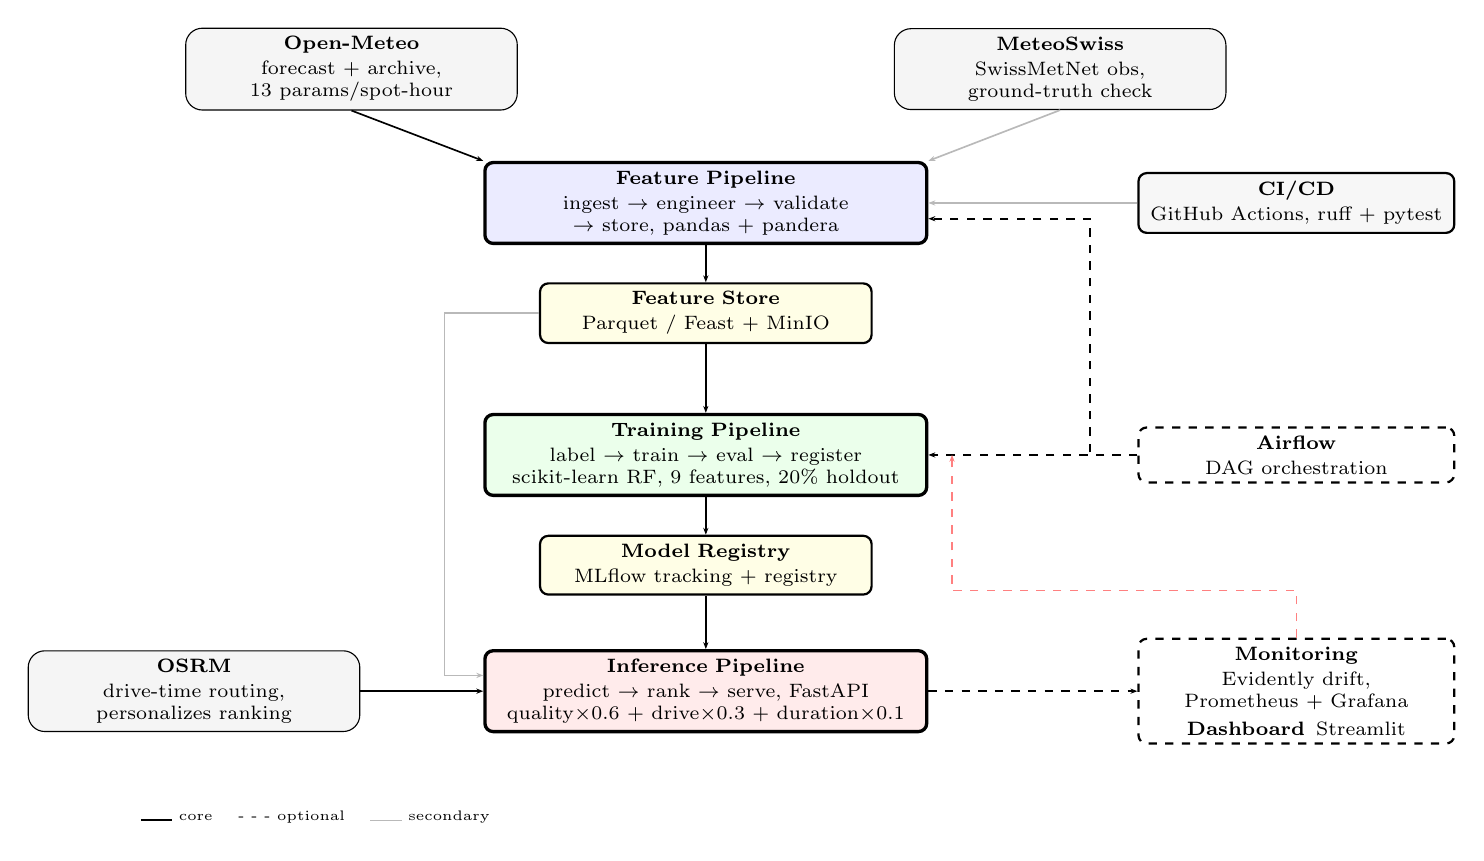
\begin{tikzpicture}[x=1cm, y=1cm, every node/.style={font=\scriptsize},
    src/.style={draw, rounded corners=6pt, fill=gray!8,
                text width=4.0cm, align=center, inner sep=3pt},
    pipe/.style={draw, very thick, rounded corners=3pt,
                 text width=5.4cm, align=center, inner sep=3pt},
    svc/.style={draw, thick, rounded corners=3pt, fill=yellow!10,
                text width=4.0cm, align=center, inner sep=3pt},
    opt/.style={draw, thick, dashed, rounded corners=3pt,
                text width=3.8cm, align=center, inner sep=3pt},
    plat/.style={draw, thick, rounded corners=3pt, fill=gray!6,
                 text width=3.8cm, align=center, inner sep=3pt},
    arr/.style={-{Stealth[length=2.5pt]}, semithick},
    darr/.style={-{Stealth[length=2.5pt]}, semithick, dashed},
  ]

  % ── Data sources (top, above Feature Pipeline) ──
  \node[src] (om) at (2.5, 5.5) {%
    \textbf{Open-Meteo}\\[1pt]
    \detail{forecast + archive, 13 params/spot-hour}};

  \node[src] (ms) at (11.5, 5.5) {%
    \textbf{MeteoSwiss}\\[1pt]
    \detail{SwissMetNet obs, ground-truth check}};

  % ── OSRM (left of Inference, feeds ranking) ──
  \node[src] (osrm) at (0.5, -2.4) {%
    \textbf{OSRM}\\[1pt]
    \detail{drive-time routing, personalizes ranking}};

  % ── FTI vertical stack (center column, x=6) ──
  \node[pipe, fill=blue!8] (F) at (7.0, 3.8) {%
    \textbf{Feature Pipeline}\\[1pt]
    \detail{ingest $\to$ engineer $\to$ validate $\to$ store, pandas + pandera}};

  \node[svc] (FS) at (7.0, 2.4) {%
    \textbf{Feature Store}\\[1pt]
    \detail{Parquet / Feast + MinIO}};

  \node[pipe, fill=green!8] (T) at (7.0, 0.6) {%
    \textbf{Training Pipeline}\\[1pt]
    \detail{label $\to$ train $\to$ eval $\to$ register}\\
    \detail{scikit-learn RF, 9 features, 20\% holdout}};

  \node[svc] (MR) at (7.0, -0.8) {%
    \textbf{Model Registry}\\[1pt]
    \detail{MLflow tracking + registry}};

  \node[pipe, fill=red!8] (I) at (7.0, -2.4) {%
    \textbf{Inference Pipeline}\\[1pt]
    \detail{predict $\to$ rank $\to$ serve, FastAPI}\\
    \detail{quality$\times$0.6 + drive$\times$0.3 + duration$\times$0.1}};

  % ── Platform services (right column, x=14.5) ──
  \node[plat] (cicd) at (14.5, 3.8) {\textbf{CI/CD}\\[1pt] \detail{GitHub Actions, ruff + pytest}};
  \node[opt]  (orch) at (14.5, 0.6) {\textbf{Airflow}\\[1pt] \detail{DAG orchestration}};
  \node[opt] (mon) at (14.5, -2.4) {%
    \textbf{Monitoring}\\[1pt]
    \detail{Evidently drift, Prometheus + Grafana}\\[2pt]
    \textbf{Dashboard}\, \detail{Streamlit}};

  % ── ARROWS: Data → FTI ──
  \draw[arr] (om.south) -- (F.north west);
  \draw[arr, gray!55] (ms.south) -- (F.north east);
  \draw[arr] (osrm.east) -- (I.west);

  % ── ARROWS: FTI vertical flow ──
  \draw[arr] (F.south)  -- (FS.north);
  \draw[arr] (FS.south) -- (T.north);
  \draw[arr] (T.south)  -- (MR.north);
  \draw[arr] (MR.south) -- (I.north);

  % Feature Store also feeds Inference (bypass arc, left side)
  \draw[arr, gray!55] (FS.west) -- ++(-1.2,0)
       |- ([yshift=2mm]I.west);

  % ── ARROWS: FTI → Platform ──
  \draw[darr] (I.east) -- (mon.west);

  % CI/CD tests pipelines
  \draw[arr, gray!55] (cicd.west) -- (F.east);
  % Airflow orchestrates Feature + Training DAGs (dashed, optional)
  \draw[darr] (orch.west) -- ++(-0.6,0) |- ([yshift=-2mm]F.east);
  \draw[darr] (orch.west) -- (T.east);

  % Drift triggers retraining (feedback loop)
  \draw[darr, red!50] (mon.north) -- ++(0,0.6)
       -| ([xshift=3mm]T.east);

  % ── Legend ──
  \node[anchor=north west, font=\tiny] at (-0.3, -3.8)
       {{\rule{0.4cm}{0.8pt}} core \quad {- - -} optional
        \quad {\color{gray!55}\rule{0.4cm}{0.4pt}} secondary};
\end{tikzpicture}
\end{center}

\smallskip
\noindent
Each pipeline maps to a sub-package in \texttt{src/foehncast/};
an optional GCP Cloud Run deployment (europe-west6) mirrors the
local Docker Compose stack.

\section{Tech Stack}

\begin{center}
\footnotesize
\begin{tabularx}{\linewidth}{l@{\hskip 4pt}X}
\toprule
\textbf{Layer} & \textbf{Technology \& Rationale} \\
\midrule
Language      & Python 3.12, \texttt{uv} package manager, hatchling build backend \\
Data          & pandas $\to$ Parquet (columnar, zero-cost local store);
                \textit{opt:} Feast feature store with MinIO S3 backend \\
Validation    & pandera schema contracts on every ingest;
                \textit{opt:} DVC for data versioning \\
Model         & scikit-learn Random Forest (interpretable, fast on tabular data);
                MLflow experiment tracking + model registry \\
Serving       & FastAPI REST API (async, auto-generated OpenAPI docs);
                \textit{opt:} Streamlit dashboard \\
Orchestration & \textit{opt:} Airflow DAGs --- thin wrappers calling pipeline modules \\
CI/CD         & GitHub Actions: lint (ruff), test (pytest), containerize;
                pre-commit hooks for local checks \\
Monitoring    & \textit{opt:} Evidently AI for drift detection;
                Prometheus + Grafana for service metrics \\
Infra         & Docker Compose with two-network isolation (frontend / backend);
                \textit{opt:} GCP Cloud Run (europe-west6) \\
\bottomrule
\end{tabularx}
\end{center}

\smallskip
\footnotesize
\textit{Italic} = optional enhancements (nice to have).
The core system is fully functional without them.
\normalsize

\end{document}
